
\documentclass[12pt]{article}
%\usepackage[finnish]{babel}
\usepackage[T1]{fontenc}
\usepackage[utf8]{inputenc}
\usepackage{amssymb}
\usepackage{amsmath}
\usepackage{graphicx}
\usepackage{hyperref}
\newcommand{\pat}{\partial}
\newcommand{\be}{\begin{equation}}
\newcommand{\ee}{\end{equation}}
\newcommand{\bea}{\begin{eqnarray}}
\newcommand{\eea}{\end{eqnarray}}
\newcommand{\abf}{{\bf a}}
\newcommand{\Zcal}{{\cal Z}_{12}}
\newcommand{\zcal}{z_{12}}
\newcommand{\Acal}{{\cal A}}
\newcommand{\Fcal}{{\cal F}}
\newcommand{\Ucal}{{\cal U}}
\newcommand{\Vcal}{{\cal V}}
\newcommand{\Ocal}{{\cal O}}
\newcommand{\Rcal}{{\cal R}}
\newcommand{\Scal}{{\cal S}}
\newcommand{\Lcal}{{\cal L}}
\newcommand{\Hcal}{{\cal H}}
\newcommand{\hsf}{{\sf h}}
\newcommand{\half}{\frac{1}{2}}
\newcommand{\Xbar}{\bar{X}}
\newcommand{\xibar}{\bar{\xi }}
\newcommand{\barh}{\bar{h}}
\newcommand{\Ubar}{\bar{\cal U}}
\newcommand{\Vbar}{\bar{\cal V}}
\newcommand{\Fbar}{\bar{F}}
\newcommand{\zbar}{\bar{z}}
\newcommand{\wbar}{\bar{w}}
\newcommand{\zbarhat}{\hat{\bar{z}}}
\newcommand{\wbarhat}{\hat{\bar{w}}}
\newcommand{\wbartilde}{\tilde{\bar{w}}}
\newcommand{\barone}{\bar{1}}
\newcommand{\bartwo}{\bar{2}}
\newcommand{\nbyn}{N \times N}
\newcommand{\repres}{\leftrightarrow}
\newcommand{\Tr}{{\rm Tr}}
\newcommand{\tr}{{\rm tr}}
\newcommand{\ninfty}{N \rightarrow \infty}
\newcommand{\unitk}{{\bf 1}_k}
\newcommand{\unitm}{{\bf 1}}
\newcommand{\zerom}{{\bf 0}}
\newcommand{\unittwo}{{\bf 1}_2}
\newcommand{\holo}{{\cal U}}
%\newcommand{\bra}{\langle}
%\newcommand{\ket}{\rangle}
\newcommand{\muhat}{\hat{\mu}}
\newcommand{\nuhat}{\hat{\nu}}
\newcommand{\rhat}{\hat{r}}
\newcommand{\phat}{\hat{\phi}}
\newcommand{\that}{\hat{t}}
\newcommand{\shat}{\hat{s}}
\newcommand{\zhat}{\hat{z}}
\newcommand{\what}{\hat{w}}
\newcommand{\sgamma}{\sqrt{\gamma}}
\newcommand{\bfE}{{\bf E}}
\newcommand{\bfB}{{\bf B}}
\newcommand{\bfM}{{\bf M}}
\newcommand{\cl} {\cal l}
\newcommand{\ctilde}{\tilde{\chi}}
\newcommand{\ttilde}{\tilde{t}}
\newcommand{\ptilde}{\tilde{\phi}}
\newcommand{\utilde}{\tilde{u}}
\newcommand{\vtilde}{\tilde{v}}
\newcommand{\wtilde}{\tilde{w}}
\newcommand{\ztilde}{\tilde{z}}
\newcommand{\ket}[1]{\vert{#1}\rangle}
\newcommand{\bra}[1]{\langle{#1}\vert}

\usepackage{listings}


\hoffset 0.5cm
\voffset -0.4cm
\evensidemargin -0.2in
\oddsidemargin -0.2in
\topmargin -0.2in
\textwidth 6.3in
\textheight 8.4in

\begin{document}

\normalsize

\baselineskip 14pt

\begin{center}
{\Large {\bf Basics of Monte Carlo Simulations 2021 \ \ \\ Report}} \\
Jake Muff
25/01/21
\end{center}
\section*{Question 1} 
Please see attached scan, detailing my answer. The scan is also in the archive.

\section*{Question 2} 
The code is attached in the same folder as this document under \lstinline{buffon.cpp}. Note that in this I did not use the standard \lstinline{rand()} 
function given in C/C++, because as discussed in class and in Numerical Recipes it is not that great. There is a better version in the \lstinline{random.h} header file included in the current
versions of C++ (not sure about C) which uses the Mersenne Twister RNG.
\\
The averages errors are shown in the \lstinline{dat1.txt} text file and plotted below. As we can see the average error goes below 0.0001 some point after $10^7$ needles. I did not calculate this explicitly because I did not know how to calculate it relatively quickly whilst still maintaining precision. 
My initial plan was to loop through the numbers 1 to $10^7$, however I quickly realised this would take a long time. 

\begin{figure}[h]
    
    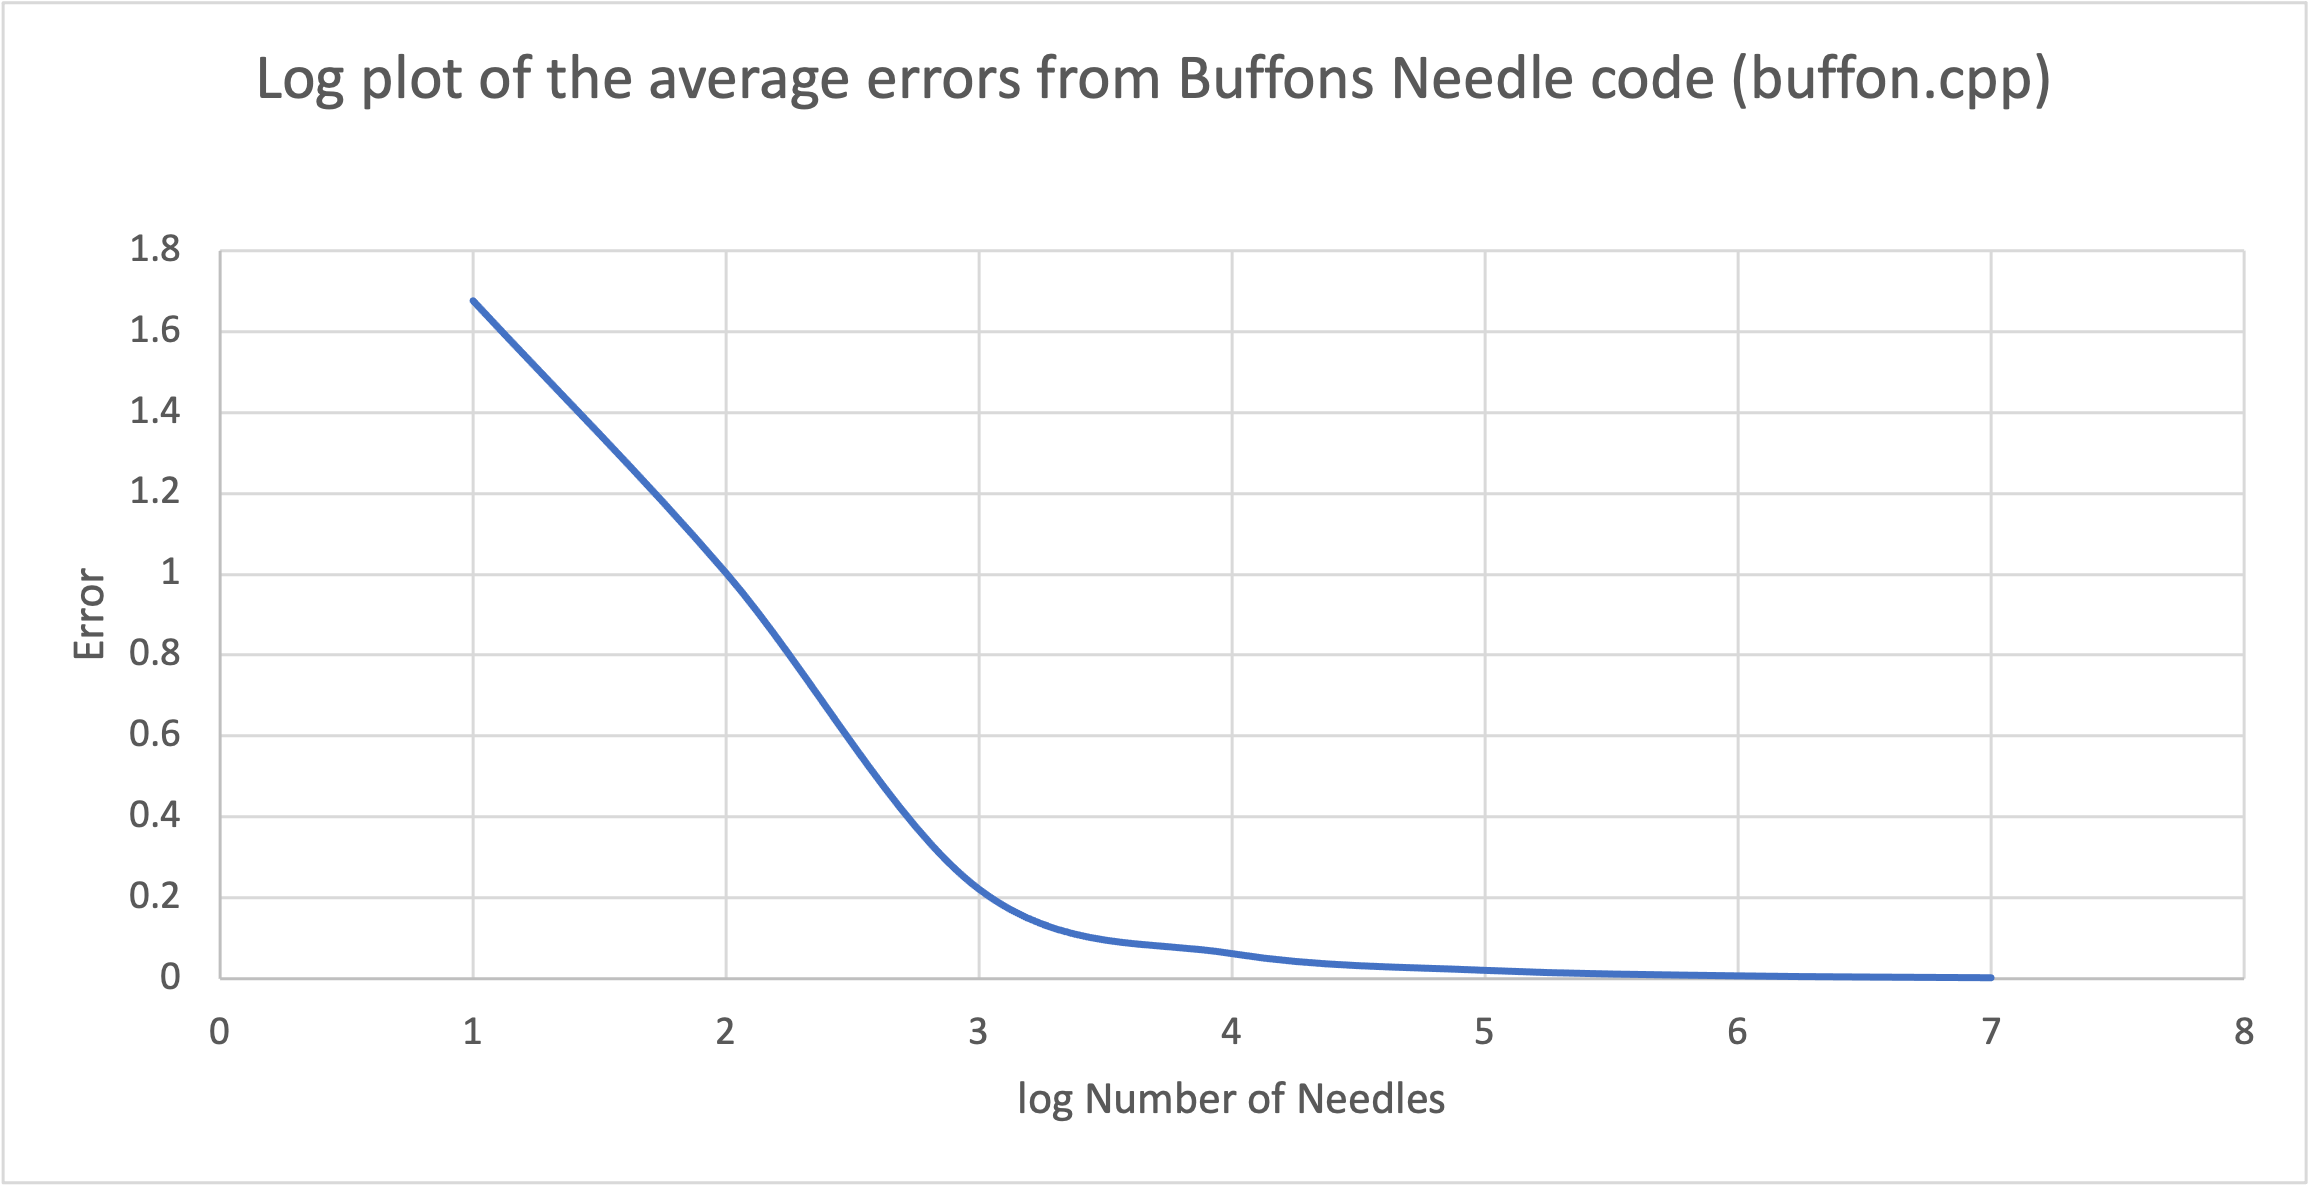
\includegraphics[width=15cm]{Picture 1.png}
    \centering
    \caption{Log plot of Averages errors as a function of the number of needles}
\end{figure}

\section*{Question 3} 
This was fairly simple, but was not without hiccups. In particular the interval of the Mersenne twister was not explicitly calculated due to its know and incredibly high period. The other two intervals were calculated and are what I expected given the conditions inputted. 
\\
For this question the header file \lstinline{rng.h} was made which includes all the relevant functions. 

\section*{Question 4} 
The plots for the LCG and Mersenne Twsiter are below. The plot for the Park Miller was not included 
because there is a bug somewhere in my code that is stopping it from writing new values to file. By inspection of the text files you can see this error immediately. 
I did not complete the 2D distribution of numbers between -1 and +1. 
\\
From the distrubutions we can see that Mersenne Twister method produces the noisest plots with the LCG seemingly repeating. 
\\
If I was to use LCG for my Buffon's needle simulation it would produces results with greater error, however I ran out of time to implement this. 

\begin{figure}[h]
    
    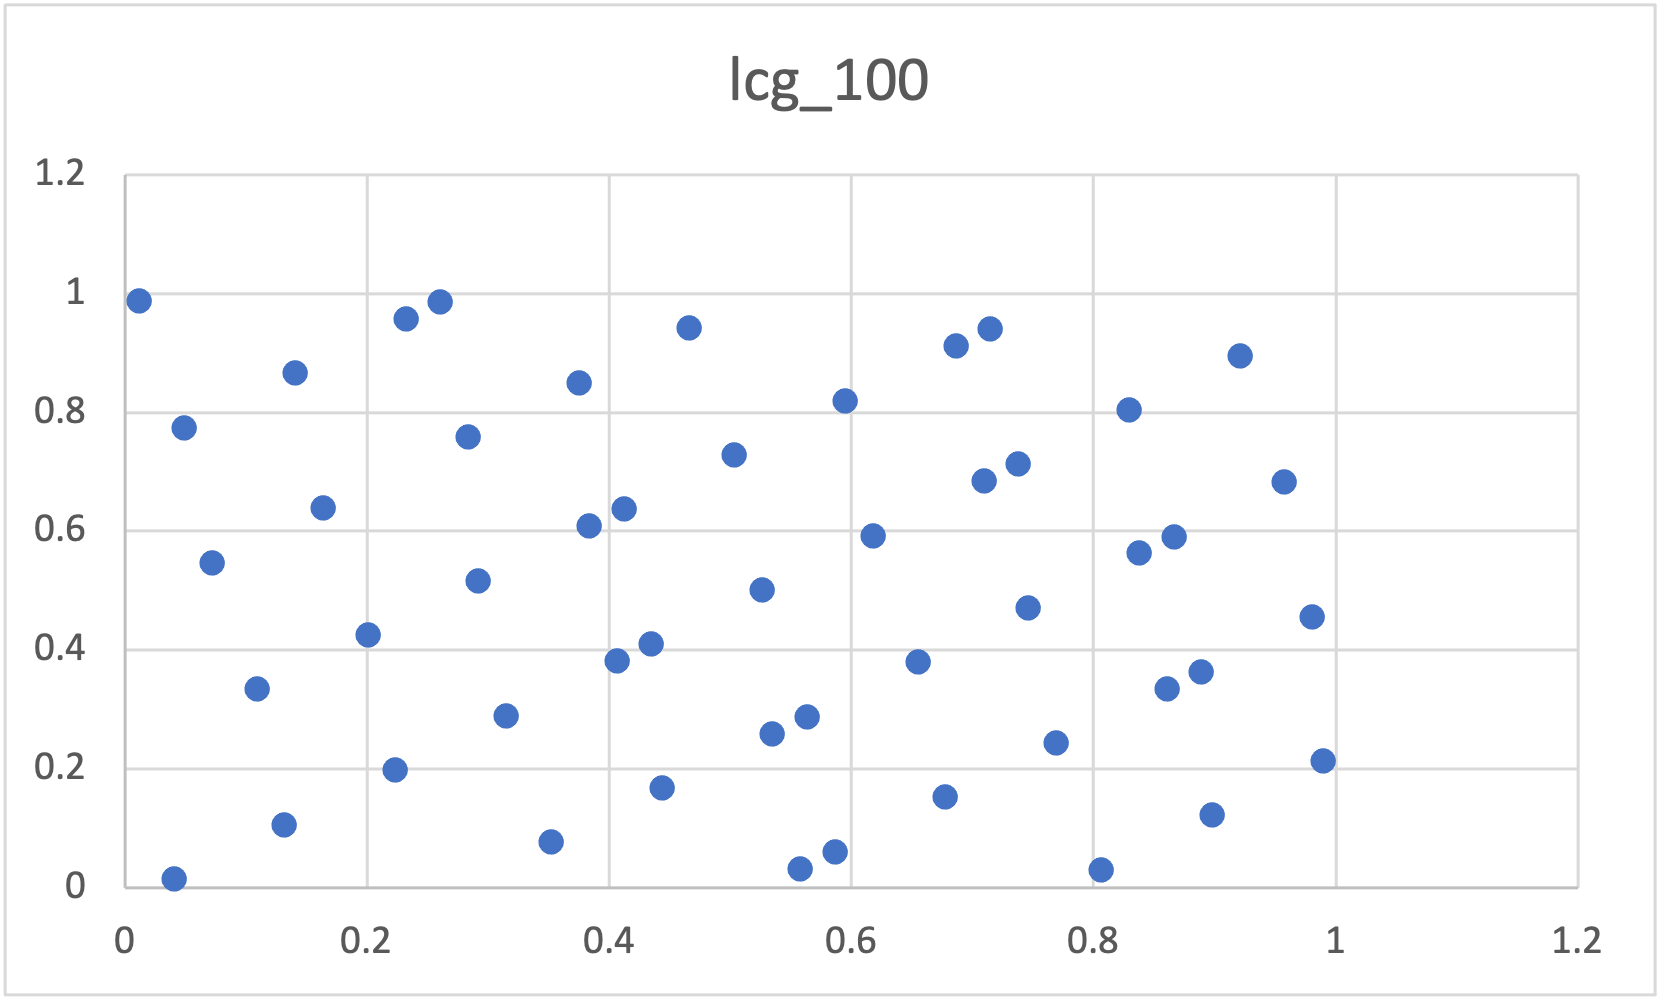
\includegraphics[width=15cm]{lcg_100.png}
    \centering
    \caption{2D points plot for LCG with 100 points}
\end{figure}
\begin{figure}[h]
    
    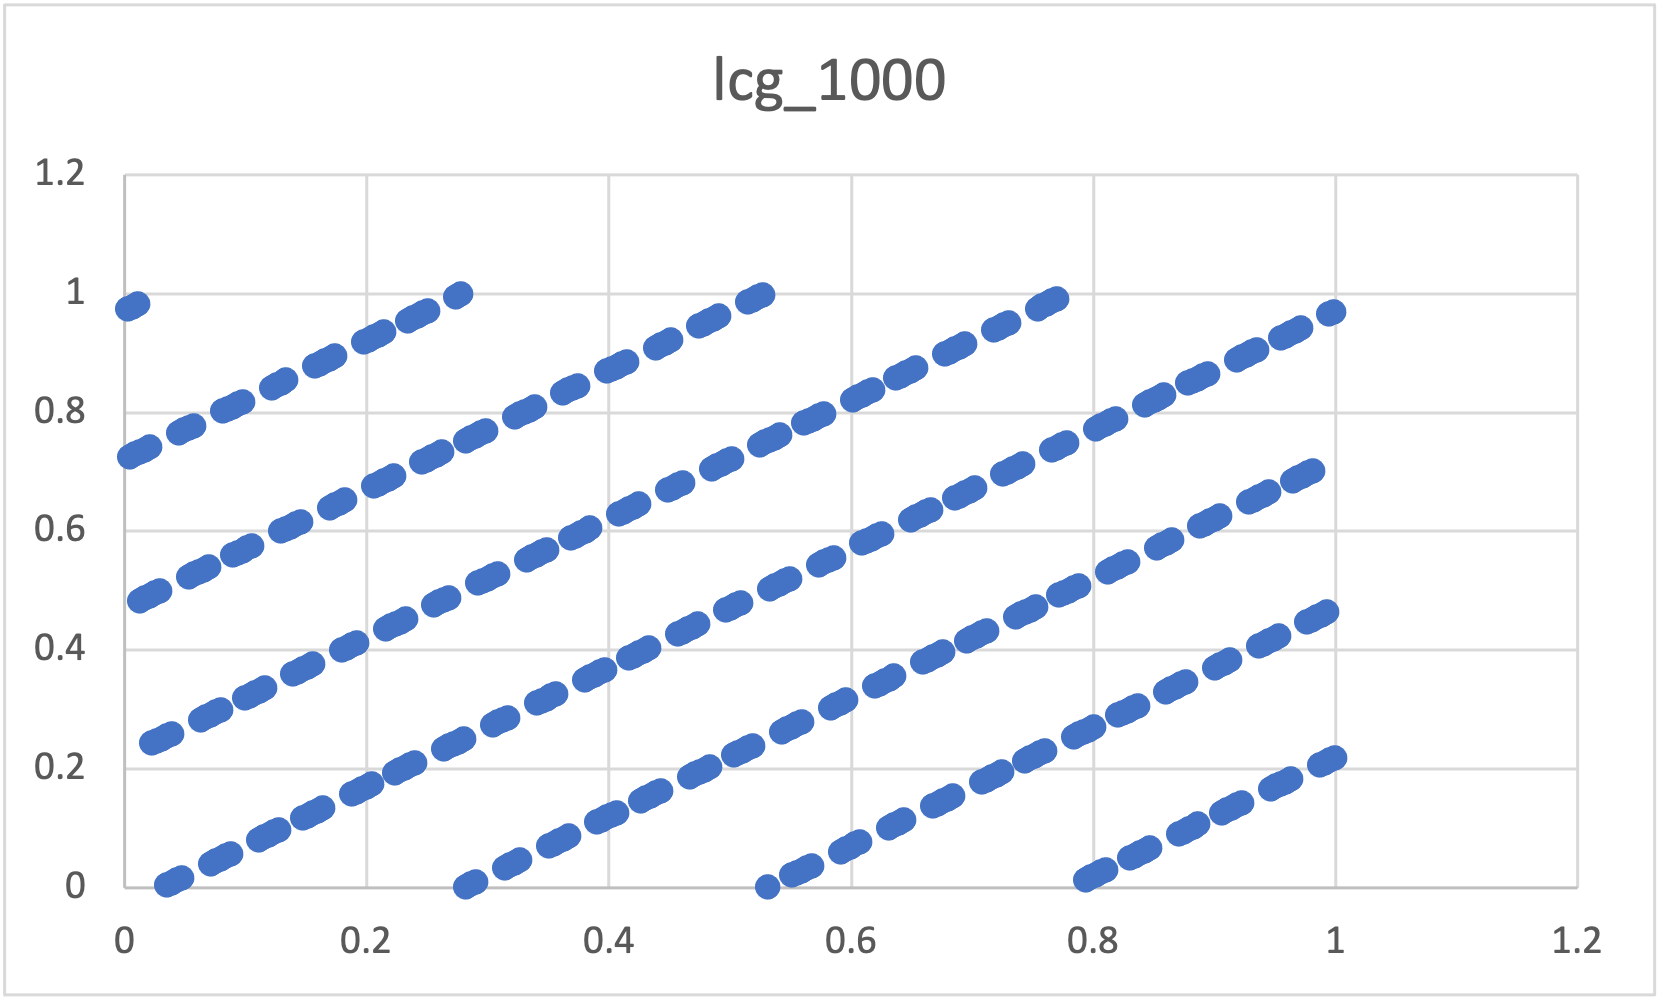
\includegraphics[width=15cm]{lcg_1000.png}
    \centering
    \caption{2D points plot for LCG with 1000 points}
\end{figure}
\begin{figure}[h]
    
    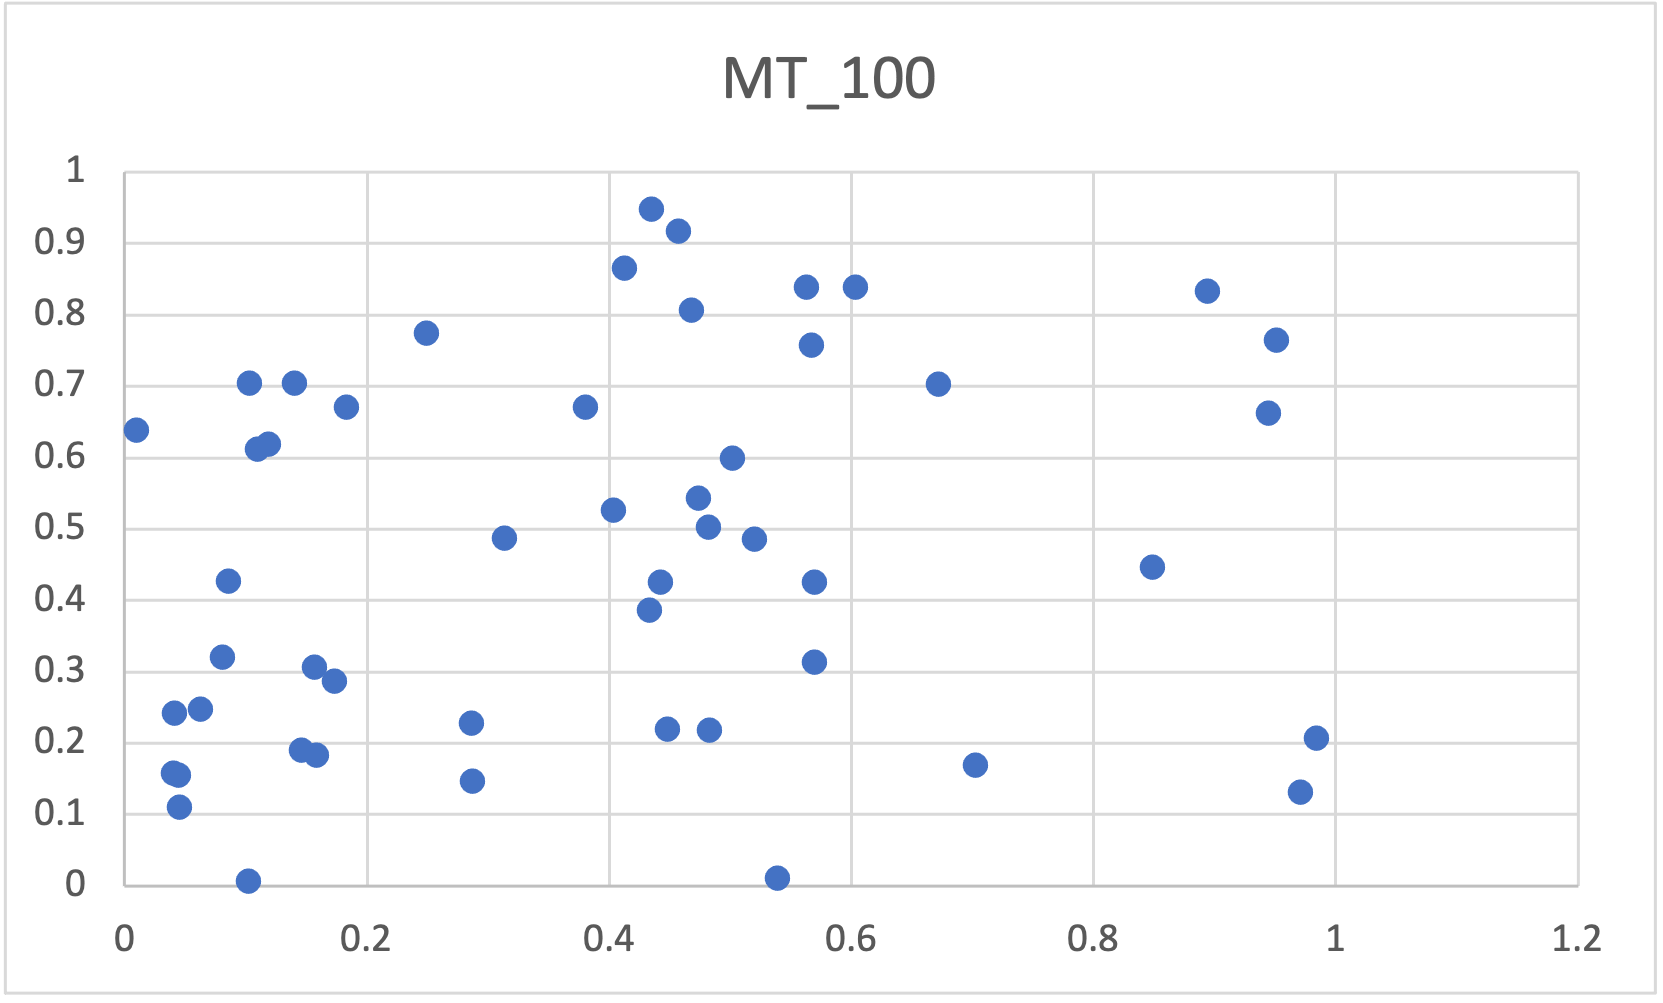
\includegraphics[width=15cm]{MT_100.png}
    \centering
    \caption{2D points plot for MT with 100 points}
\end{figure}
\begin{figure}[h]
    
    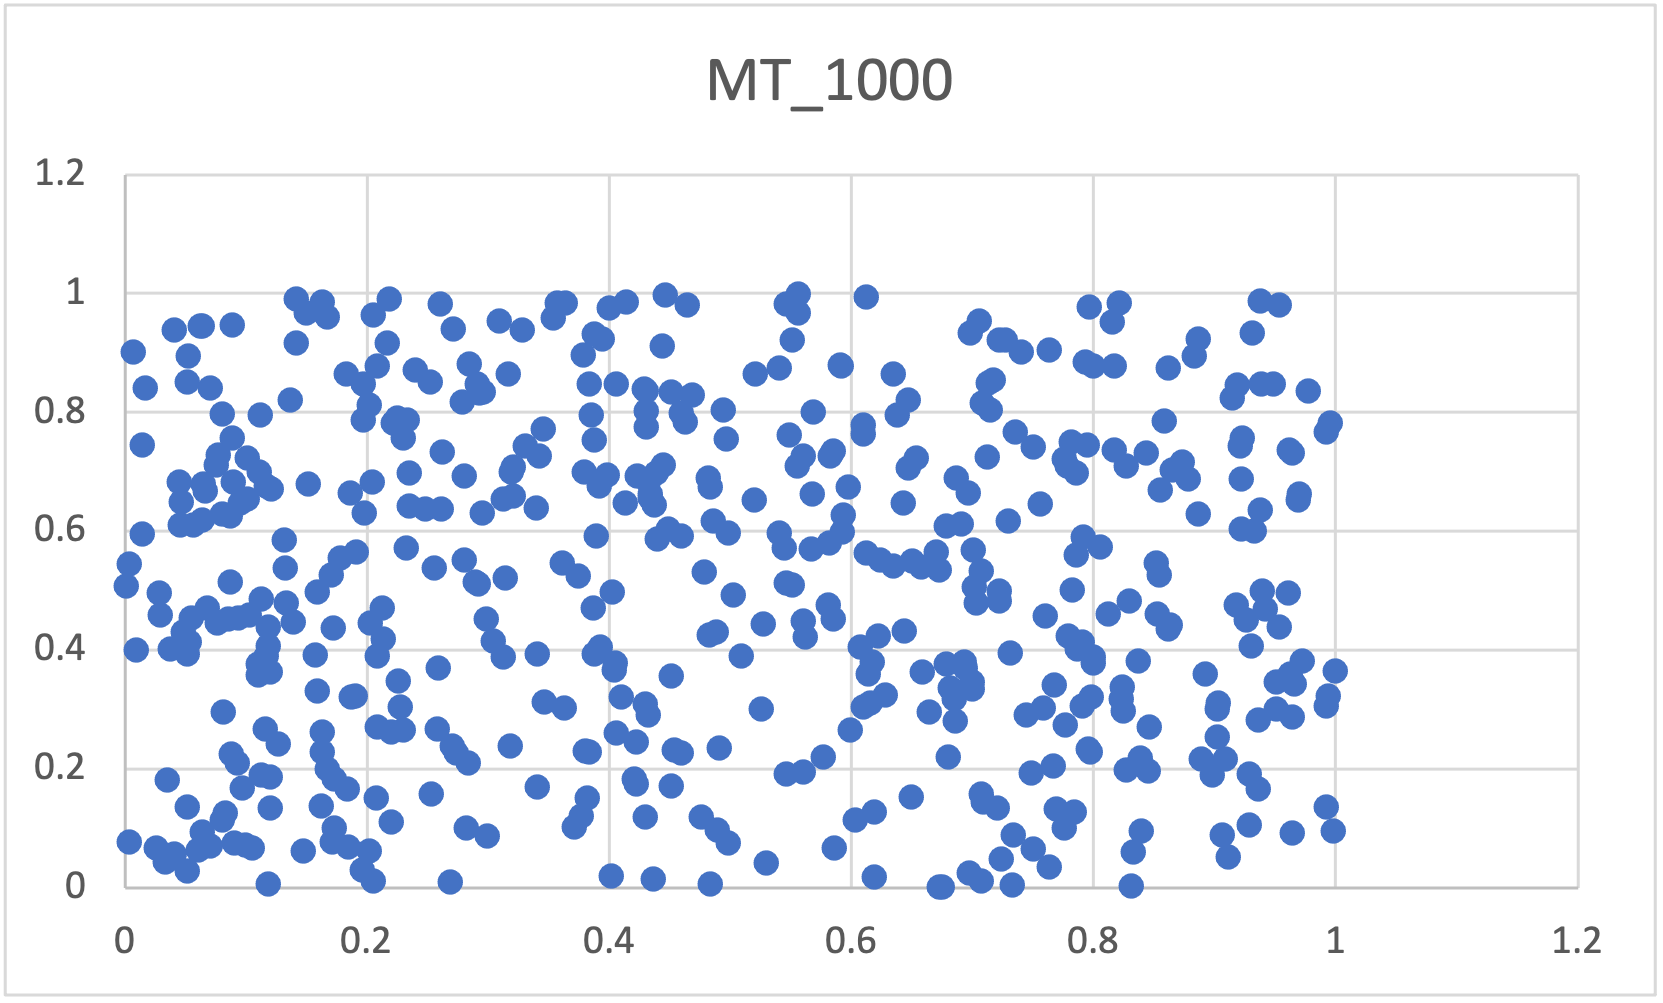
\includegraphics[width=15cm]{MT_1000.png}
    \centering
    \caption{2D points plot for MT with 1000 points}
\end{figure}

\end{document}


